\columnratio{0.55}
\begin{paracol}{2}
\switchcolumn[0]*%%%%%%%
\section{Transition}
\switchcolumn
\section{Transition}
\switchcolumn[0]*%%%%%%%
Vue offers two built-in components that can help work with transitions
and animations in response to changing state:
\switchcolumn
Vue 提供了两个内置组件,可以帮助你制作基于状态变化的过渡和动画:
\switchcolumn[0]*%%%%%%%
\begin{itemize}
\item
    \texttt{\textless{}Transition\textgreater{}} for applying animations
    when an element or component is entering and leaving the DOM. This is
    covered on this page.
\item
    \texttt{\textless{}TransitionGroup\textgreater{}} for applying
    animations when an element or component is inserted into, removed
    from, or moved within a \texttt{v-for} list. This is covered in
    \href{https://vuejs.org/guide/built-ins/transition-group.html}{the
    next chapter}.
\end{itemize}
\switchcolumn
\begin{itemize}
\item
    \texttt{\textless{}Transition\textgreater{}}
    会在一个元素或组件进入和离开 DOM 时应用动画。本章节会介绍如何使用它。
\item
    \texttt{\textless{}TransitionGroup\textgreater{}} 会在一个
    \texttt{v-for}
    列表中的元素或组件被插入,移动,或移除时应用动画。我们将在\href{https://cn.vuejs.org/guide/built-ins/transition-group.html}{下一章节}中介绍。
\end{itemize} 
\switchcolumn[0]*%%%%%%%
Aside from these two components, we can also apply animations in Vue
using other techniques such as toggling CSS classes or state-driven
animations via style bindings. These additional techniques are covered
in the \href{https://vuejs.org/guide/extras/animation.html}{Animation
Techniques} chapter.
\switchcolumn
除了这两个组件,我们也可以通过其他技术手段来应用动画,比如切换 CSS class
或用状态绑定样式来驱动动画。这些其他的方法会在\href{https://cn.vuejs.org/guide/extras/animation.html}{动画技巧}章节中展开。
\switchcolumn[0]*%%%%%%%
\subsection{The \textless Transition\textgreater{} Component}
\switchcolumn
\subsection{\textless Transition\textgreater{} 组件}
\switchcolumn[0]*%%%%%%%
\texttt{\textless{}Transition\textgreater{}} is a built-in component:
this means it is available in any component's template without having to
register it. It can be used to apply enter and leave animations on
elements or components passed to it via its default slot. The enter or
leave can be triggered by one of the following:
\switchcolumn
\texttt{\textless{}Transition\textgreater{}}
是一个内置组件,这意味着它在任意别的组件中都可以被使用,无需注册。它可以将进入和离开动画应用到通过默认插槽传递给它的元素或组件上。进入或离开可以由以下的条件之一触发:
\switchcolumn[0]*%%%%%%%
\begin{itemize}
\item
  Conditional rendering via \texttt{v-if}
\item
  Conditional display via \texttt{v-show}
\item
  Dynamic components toggling via the
  \texttt{\textless{}component\textgreater{}} special element
\item
  Changing the special \texttt{key} attribute
\end{itemize}
\switchcolumn
\begin{itemize}
\item
  由 \texttt{v-if} 所触发的切换
\item
  由 \texttt{v-show} 所触发的切换
\item
  由特殊元素 \texttt{\textless{}component\textgreater{}} 切换的动态组件
\item
  改变特殊的 \texttt{key} 属性
\end{itemize}
\switchcolumn[0]*%%%%%%%
This is an example of the most basic usage:
\switchcolumn
以下是最基本用法的示例:
\switchcolumn[0]*%%%%%%%
\begin{codeHtml}
<button @click="show = !show">Toggle</button>
<Transition>
  <p v-if="show">hello</p>
</Transition>
\end{codeHtml}
\switchcolumn
\begin{codeHtml}
<button @click="show = !show">Toggle</button>
<Transition>
  <p v-if="show">hello</p>
</Transition>
\end{codeHtml}
\switchcolumn[0]*%%%%%%%
\begin{codeCss}
/* 下面我们会解释这些 class 是做什么的 */
.v-enter-active,
.v-leave-active {
  transition: opacity 0.5s ease;
}
.v-enter-from,
.v-leave-to {
  opacity: 0;
}
\end{codeCss}
\switchcolumn
\begin{codeCss}
/* 下面我们会解释这些 class 是做什么的 */
.v-enter-active,
.v-leave-active {
  transition: opacity 0.5s ease;
}
.v-enter-from,
.v-leave-to {
  opacity: 0;
}
\end{codeCss}
\switchcolumn[0]*%%%%%%%
\href{https://play.vuejs.org/\#eNpVkEFuwyAQRa8yZZNWqu1sunFJ1N4hSzYUjRNUDAjGVJHluxcCipIV/OG/pxEr+/a+TwuykfGogvYEEWnxR2H17F0gWCHgBBtMwc2wy9WdsMIqZ2OuXtwfHErhlcKCb8LyoVoynwPh7I0kzAmA/yxEzsKXMlr9HgRr9Es5BTue3PlskA+1VpFTkDZq0i3niYfU6anRmbqgMY4PZeH8OjwBfHhYIMdIV1OuferQEoZOKtIJ328TgzJhm8BabHR3jeC8VJqusO8/IqCM+CnsVqR3V/mfRxO5amnkCPuK5B+6rcG2fydshks=}{Try
it in the Playground}
\switchcolumn
\href{https://play.vuejs.org/\#eNpVkEFuwyAQRa8yZZNWqu1sunFJ1N4hSzYUjRNUDAjGVJHluxcCipIV/OG/pxEr+/a+TwuykfGogvYEEWnxR2H17F0gWCHgBBtMwc2wy9WdsMIqZ2OuXtwfHErhlcKCb8LyoVoynwPh7I0kzAmA/yxEzsKXMlr9HgRr9Es5BTue3PlskA+1VpFTkDZq0i3niYfU6anRmbqgMY4PZeH8OjwBfHhYIMdIV1OuferQEoZOKtIJ328TgzJhm8BabHR3jeC8VJqusO8/IqCM+CnsVqR3V/mfRxO5amnkCPuK5B+6rcG2fydshks=}{在演练场中尝试一下}
\switchcolumn[0]*%%%%%%%
\begin{vueQuote}{TIP}
\texttt{\textless{}Transition\textgreater{}} only supports a single
element or component as its slot content. If the content is a component,
the component must also have only one single root element.
\end{vueQuote} 
\switchcolumn
\begin{vueQuote}{TIP}
\texttt{\textless{}Transition\textgreater{}}
仅支持单个元素或组件作为其插槽内容。如果内容是一个组件,这个组件必须仅有一个根元素。
\end{vueQuote} 
\switchcolumn[0]*%%%%%%%
When an element in a \texttt{\textless{}Transition\textgreater{}}
component is inserted or removed, this is what happens:
\switchcolumn
当一个 \texttt{\textless{}Transition\textgreater{}}
组件中的元素被插入或移除时,会发生下面这些事情:
\switchcolumn[0]*%%%%%%%
\begin{enumerate}
\item
  Vue will automatically sniff whether the target element has CSS
  transitions or animations applied. If it does, a number of
  \href{https://vuejs.org/guide/built-ins/transition.html\#transition-classes}{CSS
  transition classes} will be added / removed at appropriate timings.
\item
  If there are listeners for
  \href{https://vuejs.org/guide/built-ins/transition.html\#javascript-hooks}{JavaScript
  hooks}, these hooks will be called at appropriate timings.
\item
  If no CSS transitions / animations are detected and no JavaScript
  hooks are provided, the DOM operations for insertion and/or removal
  will be executed on the browser's next animation frame.
\end{enumerate}
\switchcolumn
\begin{enumerate}
\item
  Vue 会自动检测目标元素是否应用了 CSS 过渡或动画。如果是,则一些
  \href{https://cn.vuejs.org/guide/built-ins/transition.html\#transition-classes}{CSS
  过渡 class} 会在适当的时机被添加和移除。
\item
  如果有作为监听器的
  \href{https://cn.vuejs.org/guide/built-ins/transition.html\#javascript-hooks}{JavaScript
  钩子},这些钩子函数会在适当时机被调用。
\item
  如果没有探测到 CSS 过渡或动画、也没有提供 JavaScript 钩子,那么 DOM
  的插入、删除操作将在浏览器的下一个动画帧后执行。
\end{enumerate}
\switchcolumn[0]*%%%%%%%
\subsection{CSS-Based Transitions}
\switchcolumn
\subsection{基于 CSS 的过渡效果}
\switchcolumn[0]*%%%%%%%
\subsubsection{Transition Classes}
\switchcolumn
\subsubsection{CSS 过渡 class}
\switchcolumn[0]*%%%%%%%
There are six classes applied for enter / leave transitions.
\switchcolumn
一共有 6 个应用于进入与离开过渡效果的 CSS class。
\end{paracol}

\begin{center} 
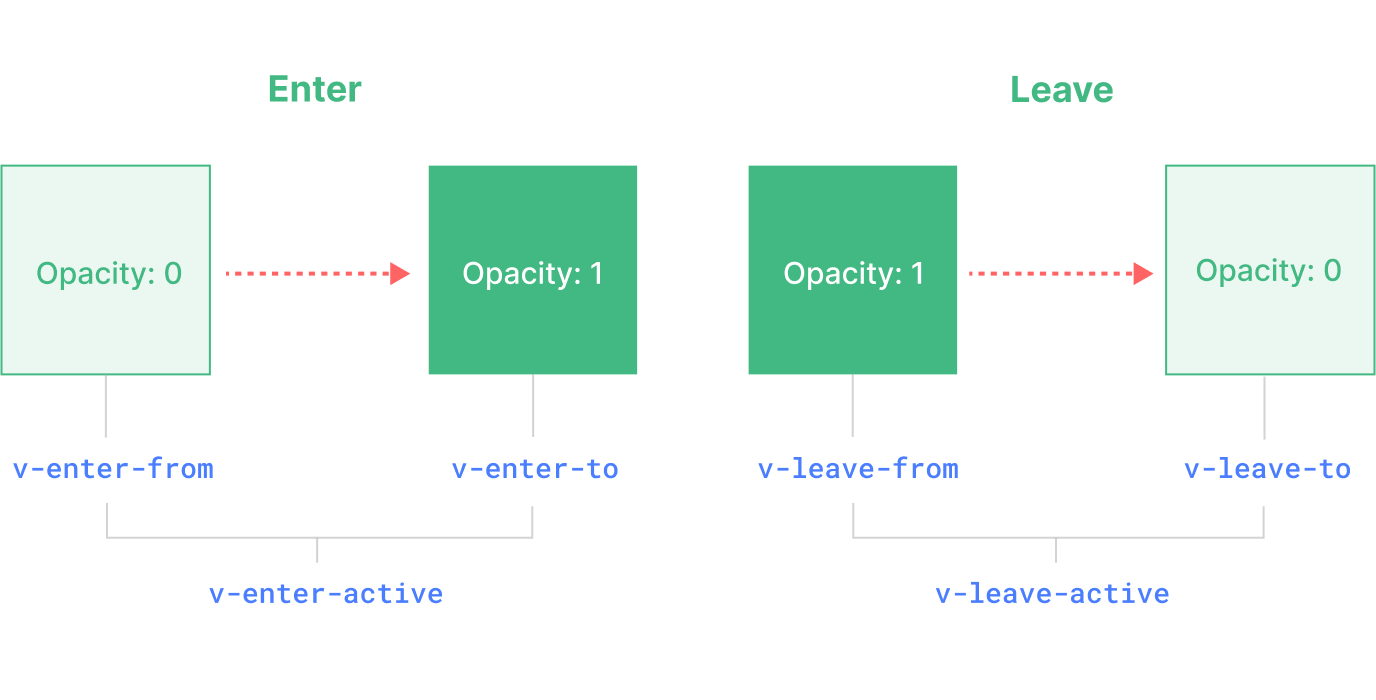
\includegraphics{./img/transition-classes.f0f7b3c9.png} 
\end{center}

\columnratio{0.55}
\begin{paracol}{2}
 
\switchcolumn[0]*%%%%%%%
\begin{enumerate}
\item
  \texttt{v-enter-from}: Starting state for enter. Added before the
  element is inserted, removed one frame after the element is inserted.
\item
  \texttt{v-enter-active}: Active state for enter. Applied during the
  entire entering phase. Added before the element is inserted, removed
  when the transition/animation finishes. This class can be used to
  define the duration, delay and easing curve for the entering
  transition.
\item
  \texttt{v-enter-to}: Ending state for enter. Added one frame after the
  element is inserted (at the same time \texttt{v-enter-from} is
  removed), removed when the transition/animation finishes.
\item
  \texttt{v-leave-from}: Starting state for leave. Added immediately
  when a leaving transition is triggered, removed after one frame.
\item
  \texttt{v-leave-active}: Active state for leave. Applied during the
  entire leaving phase. Added immediately when a leaving transition is
  triggered, removed when the transition/animation finishes. This class
  can be used to define the duration, delay and easing curve for the
  leaving transition.
\item
  \texttt{v-leave-to}: Ending state for leave. Added one frame after a
  leaving transition is triggered (at the same time
  \texttt{v-leave-from} is removed), removed when the
  transition/animation finishes.
\end{enumerate}
\switchcolumn
\begin{enumerate}
\item
  \texttt{v-enter-from}:进入动画的起始状态。在元素插入之前添加,在元素插入完成后的下一帧移除。
\item
  \texttt{v-enter-active}:进入动画的生效状态。应用于整个进入动画阶段。在元素被插入之前添加,在过渡或动画完成之后移除。这个
  class 可以被用来定义进入动画的持续时间、延迟与速度曲线类型。
\item
  \texttt{v-enter-to}:进入动画的结束状态。在元素插入完成后的下一帧被添加
  (也就是 \texttt{v-enter-from}
  被移除的同时),在过渡或动画完成之后移除。
\item
  \texttt{v-leave-from}:离开动画的起始状态。在离开过渡效果被触发时立即添加,在一帧后被移除。
\item
  \texttt{v-leave-active}:离开动画的生效状态。应用于整个离开动画阶段。在离开过渡效果被触发时立即添加,在过渡或动画完成之后移除。这个
  class 可以被用来定义离开动画的持续时间、延迟与速度曲线类型。
\item
  \texttt{v-leave-to}:离开动画的结束状态。在一个离开动画被触发后的下一帧被添加
  (也就是 \texttt{v-leave-from}
  被移除的同时),在过渡或动画完成之后移除。
\end{enumerate}
\switchcolumn[0]*%%%%%%%
\texttt{v-enter-active} and \texttt{v-leave-active} give us the ability
to specify different easing curves for enter / leave transitions, which
we'll see an example of in the following sections.
\switchcolumn
\texttt{v-enter-active} 和 \texttt{v-leave-active}
给我们提供了为进入和离开动画指定不同速度曲线的能力,我们将在下面的小节中看到一个示例。 
\end{paracol}

\columnratio{0.55}
\begin{paracol}{2}
 
\switchcolumn[0]*%%%%%%%
\subsubsection{Named Transitions}
\switchcolumn
\subsubsection{为过渡效果命名}
\switchcolumn[0]*%%%%%%%
A transition can be named via the \texttt{name} prop:
\switchcolumn
我们可以给 \texttt{\textless{}Transition\textgreater{}} 组件传一个
\texttt{name} prop 来声明一个过渡效果名:
\switchcolumn[0]*%%%%%%%
\begin{codeHtml}
<Transition name="fade">
  ...
</Transition>
\end{codeHtml}
\switchcolumn
\begin{codeHtml}
<Transition name="fade">
  ...
</Transition>
\end{codeHtml}
\switchcolumn[0]*%%%%%%%
For a named transition, its transition classes will be prefixed with its
name instead of \texttt{v}. For example, the applied class for the above
transition will be \texttt{fade-enter-active} instead of
\texttt{v-enter-active}. The CSS for the fade transition should look
like this:
\switchcolumn
对于一个有名字的过渡效果,对它起作用的过渡 class 会以其名字而不是
\texttt{v} 作为前缀。比如,上方例子中被应用的 class 将会是
\texttt{fade-enter-active} 而不是
\texttt{v-enter-active}。这个``fade''过渡的 class 应该是这样:
\switchcolumn[0]*%%%%%%%
\begin{codeCss}
.fade-enter-active,
.fade-leave-active {
  transition: opacity 0.5s ease;
}
.fade-enter-from,
.fade-leave-to {
  opacity: 0;
}
\end{codeCss}
\switchcolumn
\begin{codeCss}
.fade-enter-active,
.fade-leave-active {
  transition: opacity 0.5s ease;
}
.fade-enter-from,
.fade-leave-to {
  opacity: 0;
}
\end{codeCss}
\end{paracol}

\columnratio{0.55}
\begin{paracol}{2}
 
\switchcolumn[0]*%%%%%%%
\subsubsection{CSS Transitions}
\switchcolumn
\subsubsection{CSS 的 transition}
\switchcolumn[0]*%%%%%%%
\texttt{\textless{}Transition\textgreater{}} is most commonly used in
combination with
\href{https://developer.mozilla.org/en-US/docs/Web/CSS/CSS_Transitions/Using_CSS_transitions}{native
CSS transitions}, as seen in the basic example above. The
\texttt{transition} CSS property is a shorthand that allows us to
specify multiple aspects of a transition, including properties that
should be animated, duration of the transition, and
\href{https://developer.mozilla.org/en-US/docs/Web/CSS/easing-function}{easing
curves}.
\switchcolumn
\texttt{\textless{}Transition\textgreater{}}
一般都会搭配\href{https://developer.mozilla.org/en-US/docs/Web/CSS/CSS_Transitions/Using_CSS_transitions}{原生
CSS 过渡}一起使用,正如你在上面的例子中所看到的那样。这个
\texttt{transition} CSS
属性是一个简写形式,使我们可以一次定义一个过渡的各个方面,包括需要执行动画的属性、持续时间和\href{https://developer.mozilla.org/en-US/docs/Web/CSS/easing-function}{速度曲线}。
\switchcolumn[0]*%%%%%%%
Here is a more advanced example that transitions multiple properties,
with different durations and easing curves for enter and leave:
\switchcolumn
下面是一个更高级的例子,它使用了不同的持续时间和速度曲线来过渡多个属性:
\switchcolumn[0]*%%%%%%%
\begin{codeHtml}
<Transition name="slide-fade">
  <p v-if="show">hello</p>
</Transition>
\end{codeHtml}
\switchcolumn
\begin{codeHtml}
<Transition name="slide-fade">
  <p v-if="show">hello</p>
</Transition>
\end{codeHtml}
\switchcolumn[0]*%%%%%%%
\begin{codeCss}
/*
  进入和离开动画可以使用不同
  持续时间和速度曲线。
*/
.slide-fade-enter-active {
  transition: all 0.3s ease-out;
}
.slide-fade-leave-active {
  transition: all 0.8s cubic-bezier(1, 0.5, 0.8, 1);
}
.slide-fade-enter-from,
.slide-fade-leave-to {
  transform: translateX(20px);
  opacity: 0;
}
\end{codeCss}
\switchcolumn
\begin{codeCss}
/*
  进入和离开动画可以使用不同
  持续时间和速度曲线。
*/
.slide-fade-enter-active {
  transition: all 0.3s ease-out;
}
.slide-fade-leave-active {
  transition: all 0.8s cubic-bezier(1, 0.5, 0.8, 1);
}
.slide-fade-enter-from,
.slide-fade-leave-to {
  transform: translateX(20px);
  opacity: 0;
}
\end{codeCss}
\switchcolumn[0]*%%%%%%%
\href{https://play.vuejs.org/\#eNqFkc9uwjAMxl/F6wXQKIVNk1AX0HbZC4zDDr2E4EK0NIkStxtDvPviFQ0OSFzyx/m+n+34kL16P+lazMpMRBW0J4hIrV9WVjfeBYIDBKzhCHVwDQySdFDZyipnY5Lu3BcsWDCk0OKosqLoKcmfLoSNN5KQbyTWLZGz8KKMVp+LKju573ivsuXKbbcG4d3oDcI9vMkNiqL3JD+AWAVpoyadGFY2yATW5nVSJj9rkspDl+v6hE/hHRrjRMEdpdfiDEkBUVxWaEWkveHj5AzO0RKGXCrSHcKBIfSPKEEaA9PJYwSUEXPX0nNlj8y6RBiUHd5AzCOodq1VvsYfjWE4G6fgEy/zMcxG17B9ZTyX8bV85C5y1S40ZX/kdj+GD1P/zVQA56XStC9h2idJI/z7huz4CxoVvE4=}{Try
it in the Playground}
\switchcolumn
\href{https://play.vuejs.org/\#eNqFkc9uwjAMxl/F6wXQKIVNk1AX0HbZC4zDDr2E4EK0NIkStxtDvPviFQ0OSFzyx/m+n+34kL16P+lazMpMRBW0J4hIrV9WVjfeBYIDBKzhCHVwDQySdFDZyipnY5Lu3BcsWDCk0OKosqLoKcmfLoSNN5KQbyTWLZGz8KKMVp+LKju573ivsuXKbbcG4d3oDcI9vMkNiqL3JD+AWAVpoyadGFY2yATW5nVSJj9rkspDl+v6hE/hHRrjRMEdpdfiDEkBUVxWaEWkveHj5AzO0RKGXCrSHcKBIfSPKEEaA9PJYwSUEXPX0nNlj8y6RBiUHd5AzCOodq1VvsYfjWE4G6fgEy/zMcxG17B9ZTyX8bV85C5y1S40ZX/kdj+GD1P/zVQA56XStC9h2idJI/z7huz4CxoVvE4=}{在演练场中尝试一下}
\end{paracol}

\columnratio{0.55}
\begin{paracol}{2}
 
\switchcolumn[0]*%%%%%%%
\subsubsection{CSS Animations}
\switchcolumn
\subsubsection{CSS 的 animation}
\switchcolumn[0]*%%%%%%%
\href{https://developer.mozilla.org/en-US/docs/Web/CSS/CSS_Animations/Using_CSS_animations}{Native
CSS animations} are applied in the same way as CSS transitions, with the
difference being that \texttt{*-enter-from} is not removed immediately
after the element is inserted, but on an \texttt{animationend} event.
\switchcolumn
\href{https://developer.mozilla.org/en-US/docs/Web/CSS/CSS_Animations/Using_CSS_animations}{原生
CSS 动画}和 CSS transition
的应用方式基本上是相同的,只有一点不同,那就是 \texttt{*-enter-from}
不是在元素插入后立即移除,而是在一个 \texttt{animationend}
事件触发时被移除。
\switchcolumn[0]*%%%%%%%
For most CSS animations, we can simply declare them under the
\texttt{*-enter-active} and \texttt{*-leave-active} classes. Here's an
example:
\switchcolumn
对于大多数的 CSS 动画,我们可以简单地在 \texttt{*-enter-active} 和
\texttt{*-leave-active} class 下声明它们。下面是一个示例:
\switchcolumn[0]*%%%%%%%
\begin{codeHtml}
<Transition name="bounce">
  <p v-if="show" style="text-align: center;">
    Hello here is some bouncy text!
  </p>
</Transition>
\end{codeHtml}
\switchcolumn
\begin{codeHtml}
<Transition name="bounce">
  <p v-if="show" style="text-align: center;">
    Hello here is some bouncy text!
  </p>
</Transition>
\end{codeHtml}
\switchcolumn[0]*%%%%%%%
\begin{codeCss}
.bounce-enter-active {
  animation: bounce-in 0.5s;
}
.bounce-leave-active {
  animation: bounce-in 0.5s reverse;
}
@keyframes bounce-in {
  0% {
    transform: scale(0);
  }
  50% {
    transform: scale(1.25);
  }
  100% {
    transform: scale(1);
  }
}
\end{codeCss}
\switchcolumn
\begin{codeCss}
.bounce-enter-active {
  animation: bounce-in 0.5s;
}
.bounce-leave-active {
  animation: bounce-in 0.5s reverse;
}
@keyframes bounce-in {
  0% {
    transform: scale(0);
  }
  50% {
    transform: scale(1.25);
  }
  100% {
    transform: scale(1);
  }
}
\end{codeCss}
\switchcolumn[0]*%%%%%%%
\href{https://play.vuejs.org/\#eNqNksGOgjAQhl9lJNmoBwRNvCAa97YP4JFLbQZsLG3TDqzG+O47BaOezCYkpfB9/0wHbsm3c4u+w6RIyiC9cgQBqXO7yqjWWU9wA4813KH2toUpo9PKVEZaExg92V/YRmBGvsN5ZcpsTGGfN4St04Iw7qg8dkTWwF5qJc/bKnnYk7hWye5gm0ZjmY0YKwDlwQsTFCnWjGiRpaPtjETG43smHPSpqh9pVQKBrjpyrfCNMilZV8Aqd5cNEF4oFVo1pgCJhtBvnjEAP6i1hRN6BBUg2BZhKHUdvMmjWhYHE9dXY/ygzN4PasqhB75djM2mQ7FUSFI9wi0GCJ6uiHYxVsFUGcgX67CpzP0lahQ9/k/kj9CjDzgG7M94rT1PLLxhQ0D+Na4AFI9QW98WEKTQOMvnLAOwDrD+wC0Xq/Ubusw/sU+QL/45hskk9z8Bddbn}{Try
it in the Playground}
\switchcolumn
\href{https://play.vuejs.org/\#eNqNksGOgjAQhl9lJNmoBwRNvCAa97YP4JFLbQZsLG3TDqzG+O47BaOezCYkpfB9/0wHbsm3c4u+w6RIyiC9cgQBqXO7yqjWWU9wA4813KH2toUpo9PKVEZaExg92V/YRmBGvsN5ZcpsTGGfN4St04Iw7qg8dkTWwF5qJc/bKnnYk7hWye5gm0ZjmY0YKwDlwQsTFCnWjGiRpaPtjETG43smHPSpqh9pVQKBrjpyrfCNMilZV8Aqd5cNEF4oFVo1pgCJhtBvnjEAP6i1hRN6BBUg2BZhKHUdvMmjWhYHE9dXY/ygzN4PasqhB75djM2mQ7FUSFI9wi0GCJ6uiHYxVsFUGcgX67CpzP0lahQ9/k/kj9CjDzgG7M94rT1PLLxhQ0D+Na4AFI9QW98WEKTQOMvnLAOwDrD+wC0Xq/Ubusw/sU+QL/45hskk9z8Bddbn}{在演练场中尝试一下}
\end{paracol}

\columnratio{0.55}
\begin{paracol}{2}
 
\switchcolumn[0]*%%%%%%%
\subsubsection{Custom Transition Classes}
\switchcolumn
\subsubsection{自定义过渡 class}
\switchcolumn[0]*%%%%%%%
You can also specify custom transition classes by passing the following
props to \texttt{\textless{}Transition\textgreater{}}:
\switchcolumn
你也可以向 \texttt{\textless{}Transition\textgreater{}} 传递以下的 props
来指定自定义的过渡 class:
\switchcolumn[0]*%%%%%%%
\begin{itemize}
\item
  \texttt{enter-from-class}
\item
  \texttt{enter-active-class}
\item
  \texttt{enter-to-class}
\item
  \texttt{leave-from-class}
\item
  \texttt{leave-active-class}
\item
  \texttt{leave-to-class}
\end{itemize}
\switchcolumn
\begin{itemize}
\item
  \texttt{enter-from-class}
\item
  \texttt{enter-active-class}
\item
  \texttt{enter-to-class}
\item
  \texttt{leave-from-class}
\item
  \texttt{leave-active-class}
\item
  \texttt{leave-to-class}
\end{itemize}
\switchcolumn[0]*%%%%%%%
These will override the conventional class names. This is especially
useful when you want to combine Vue's transition system with an existing
CSS animation library, such as
\href{https://daneden.github.io/animate.css/}{Animate.css}:
\switchcolumn
你传入的这些 class 会覆盖相应阶段的默认 class 名。这个功能在你想要在 Vue
的动画机制下集成其他的第三方 CSS 动画库时非常有用,比如
\href{https://daneden.github.io/animate.css/}{Animate.css}:
\switchcolumn[0]*%%%%%%%
\begin{codeHtml}
<!-- 假设你已经在页面中引入了 Animate.css -->
<Transition
  name="custom-classes"
  enter-active-class="animate__animated animate__tada"
  leave-active-class="animate__animated animate__bounceOutRight"
>
  <p v-if="show">hello</p>
</Transition>
\end{codeHtml}
\switchcolumn
\begin{codeHtml}
<!-- 假设你已经在页面中引入了 Animate.css -->
<Transition
  name="custom-classes"
  enter-active-class="animate__animated animate__tada"
  leave-active-class="animate__animated animate__bounceOutRight"
>
  <p v-if="show">hello</p>
</Transition>
\end{codeHtml}
\switchcolumn[0]*%%%%%%%
\href{https://play.vuejs.org/\#eNqNUctuwjAQ/BXXF9oDsZB6ogbRL6hUcbSEjLMhpn7JXtNWiH/vhqS0R3zxPmbWM+szf02pOVXgSy6LyTYhK4A1rVWwPsWM7MwydOzCuhw9mxF0poIKJoZC0D5+stUAeMRc4UkFKcYpxKcEwSenEYYM5b4ixsA2xlnzsVJ8Yj8Mt+LrbTwcHEgxwojCmNxmHYpFG2kaoxO0B2KaWjD6uXG6FCiKj00ICHmuDdoTjD2CavJBCna7KWjZrYK61b9cB5pI93P3sQYDbxXf7aHHccpVMolO7DS33WSQjPXgXJRi2Cl1xZ8nKkjxf0dBFvx2Q7iZtq94j5jKUgjThmNpjIu17ZzO0JjohT7qL+HsvohJWWNKEc/NolncKt6Goar4y/V7rg/wyw9zrLOy}{Try
it in the Playground}
\switchcolumn
\href{https://play.vuejs.org/\#eNqNUctuwjAQ/BXXF9oDsZB6ogbRL6hUcbSEjLMhpn7JXtNWiH/vhqS0R3zxPmbWM+szf02pOVXgSy6LyTYhK4A1rVWwPsWM7MwydOzCuhw9mxF0poIKJoZC0D5+stUAeMRc4UkFKcYpxKcEwSenEYYM5b4ixsA2xlnzsVJ8Yj8Mt+LrbTwcHEgxwojCmNxmHYpFG2kaoxO0B2KaWjD6uXG6FCiKj00ICHmuDdoTjD2CavJBCna7KWjZrYK61b9cB5pI93P3sQYDbxXf7aHHccpVMolO7DS33WSQjPXgXJRi2Cl1xZ8nKkjxf0dBFvx2Q7iZtq94j5jKUgjThmNpjIu17ZzO0JjohT7qL+HsvohJWWNKEc/NolncKt6Goar4y/V7rg/wyw9zrLOy}{在演练场中尝试一下}
\end{paracol}

\columnratio{0.55}
\begin{paracol}{2}
 
\switchcolumn[0]*%%%%%%%
\subsubsection{Using Transitions and Animations Together}
\switchcolumn
\subsubsection{同时使用 transition 和 animation}
\switchcolumn[0]*%%%%%%%
Vue needs to attach event listeners in order to know when a transition
has ended. It can either be \texttt{transitionend} or
\texttt{animationend}, depending on the type of CSS rules applied. If
you are only using one or the other, Vue can automatically detect the
correct type.
\switchcolumn
Vue 需要附加事件监听器,以便知道过渡何时结束。可以是
\texttt{transitionend} 或 \texttt{animationend},这取决于你所应用的 CSS
规则。如果你仅仅使用二者的其中之一,Vue 可以自动探测到正确的类型。
\switchcolumn[0]*%%%%%%%
However, in some cases you may want to have both on the same element,
for example having a CSS animation triggered by Vue, along with a CSS
transition effect on hover. In these cases, you will have to explicitly
declare the type you want Vue to care about by passing the \texttt{type}
prop, with a value of either \texttt{animation} or \texttt{transition}:
\switchcolumn
然而在某些场景中,你或许想要在同一个元素上同时使用它们两个。举例来说,Vue
触发了一个 CSS 动画,同时鼠标悬停触发另一个 CSS
过渡。此时你需要显式地传入 \texttt{type} prop 来声明,告诉 Vue
需要关心哪种类型,传入的值是 \texttt{animation} 或 \texttt{transition}:
\switchcolumn[0]*%%%%%%%
\begin{codeHtml}
<Transition type="animation">...</Transition>
\end{codeHtml}
\switchcolumn
\begin{codeHtml}
<Transition type="animation">...</Transition>
\end{codeHtml}
\end{paracol}

\columnratio{0.55}
\begin{paracol}{2}
 
\switchcolumn[0]*%%%%%%%
\subsubsection{Nested Transitions and Explicit Transition Durations}
\switchcolumn
\subsubsection{深层级过渡与显式过渡时长}
\switchcolumn[0]*%%%%%%%
Although the transition classes are only applied to the direct child
element in \texttt{\textless{}Transition\textgreater{}}, we can
transition nested elements using nested CSS selectors:
\switchcolumn
尽管过渡 class 仅能应用在 \texttt{\textless{}Transition\textgreater{}}
的直接子元素上,我们还是可以使用深层级的 CSS
选择器,在深层级的元素上触发过渡效果。
\switchcolumn[0]*%%%%%%%
\begin{codeHtml}
<Transition name="nested">
  <div v-if="show" class="outer">
    <div class="inner">
      Hello
    </div>
  </div>
</Transition>
\end{codeHtml}
\switchcolumn
\begin{codeHtml}
<Transition name="nested">
  <div v-if="show" class="outer">
    <div class="inner">
      Hello
    </div>
  </div>
</Transition>
\end{codeHtml}
\switchcolumn[0]*%%%%%%%
\begin{codeCss}
/* 应用于嵌套元素的规则 */
.nested-enter-active .inner,
.nested-leave-active .inner {
  transition: all 0.3s ease-in-out;
}
.nested-enter-from .inner,
.nested-leave-to .inner {
  transform: translateX(30px);
  opacity: 0;
}
/* ... 省略了其他必要的 CSS */
\end{codeCss}
\switchcolumn
\begin{codeCss}
/* 应用于嵌套元素的规则 */
.nested-enter-active .inner,
.nested-leave-active .inner {
  transition: all 0.3s ease-in-out;
}
.nested-enter-from .inner,
.nested-leave-to .inner {
  transform: translateX(30px);
  opacity: 0;
}
/* ... 省略了其他必要的 CSS */
\end{codeCss}
\switchcolumn[0]*%%%%%%%
We can even add a transition delay to the nested element on enter, which
creates a staggered enter animation sequence:
\switchcolumn
我们甚至可以在深层元素上添加一个过渡延迟,从而创建一个带渐进延迟的动画序列:
\switchcolumn[0]*%%%%%%%
\begin{codeCss}
/* 延迟嵌套元素的进入以获得交错效果 */
.nested-enter-active .inner {
  transition-delay: 0.25s;
}
\end{codeCss}
\switchcolumn
\begin{codeCss}
/* 延迟嵌套元素的进入以获得交错效果 */
.nested-enter-active .inner {
  transition-delay: 0.25s;
}
\end{codeCss}
\switchcolumn[0]*%%%%%%%
However, this creates a small issue. By default, the
\texttt{\textless{}Transition\textgreater{}} component attempts to
automatically figure out when the transition has finished by listening
to the \textbf{first} \texttt{transitionend} or \texttt{animationend}
event on the root transition element. With a nested transition, the
desired behavior should be waiting until the transitions of all inner
elements have finished.
\switchcolumn
然而,这会带来一个小问题。默认情况下,\texttt{\textless{}Transition\textgreater{}}
组件会通过监听过渡根元素上的\textbf{第一个} \texttt{transitionend} 或者
\texttt{animationend}
事件来尝试自动判断过渡何时结束。而在嵌套的过渡中,期望的行为应该是等待所有内部元素的过渡完成。
\switchcolumn[0]*%%%%%%%
In such cases you can specify an explicit transition duration (in
milliseconds) using the \texttt{duration} prop on the
\texttt{\textless{}transition\textgreater{}} component. The total
duration should match the delay plus transition duration of the inner
element:
\switchcolumn
在这种情况下,你可以通过向 \texttt{\textless{}Transition\textgreater{}}
组件传入 \texttt{duration} prop 来显式指定过渡的持续时间
(以毫秒为单位)。总持续时间应该匹配延迟加上内部元素的过渡持续时间:
\switchcolumn[0]*%%%%%%%
\begin{codeHtml}
<Transition :duration="550">...</Transition>
\end{codeHtml}
\switchcolumn
\begin{codeHtml}
<Transition :duration="550">...</Transition>
\end{codeHtml}
\switchcolumn[0]*%%%%%%%
\href{https://play.vuejs.org/\#eNqVVd9v0zAQ/leO8LAfrE3HNKSFbgKmSYMHQNAHkPLiOtfEm2NHttN2mvq/c7bTNi1jgFop9t13d9995ziPyfumGc5bTLJkbLkRjQOLrm2uciXqRhsHj2BwBiuYGV3DAUEPcpUrrpUlaKUXcOkBh860eJSrcRqzUDxtHNaNZA5pBzCets5pBe+4FPz+Mk+66Bf+mSdXE12WEsdphMWQiWHKCicoLCtaw/yKIs/PR3kCitVIG4XWYUEJfATFFGIO84GYdRUIyCWzlra6dWg2wA66dgqlts7c+d8tSqk34JTQ6xqb9TjdUiTDOO21TFvrHqRfDkPpExiGKvBITjdl/L40ulVFBi8R8a3P17CiEKrM4GzULIOlFmpQoSgrl8HpKFpX3kFZu2y0BNhJxznvwaJCA1TEYcC4E3MkKp1VIptjZ43E3KajDJiUMBqeWUBmcUBUqJGYOT2GAiV7gJAA9Iy4GyoBKLH2z+N0W3q/CMC2yCCkyajM63Mbc+9z9mfvZD+b071MM23qLC69+j8PvX5HQUDdMC6cL7BOTtQXCJwpas/qHhWIBdYtWGgtDWNttWTmThu701pf1W6+v1Hd8Xbz+k+VQxmv8i7Fv1HZn+g/iv2nRkjzbd6npf/Rkz49DifQ3dLZBBYOJzC4rqgCwsUbmLYlCAUVU4XsCd1NrCeRHcYXb1IJC/RX2hEYCwJTvHYVMZoavbBI09FmU+LiFSzIh0AIXy1mqZiFKaKCmVhiEVJ7GftHZTganUZ56EYLL3FykjhL195MlMM7qxXdmEGDPOG6boRE86UJVPMki+p4H01WLz4Fm78hSdBo5xXy+yfsd3bpbXny1SA1M8c82fgcMyW66L75/hmXtN44a120ktDPOL+h1bL1HCPsA42DaPdwge3HcO/TOCb2ZumQJtA15Yl65Crg84S+BdfPtL6lezY8C3GkZ7L6Bc1zNR0=}{Try
it in the Playground}
\switchcolumn
\href{https://play.vuejs.org/\#eNqVVMtu2zAQ/JWtekjiRo80cIGoStCil3yADy2gC02tJCIUKZCUncDwv3cpyrbstmgLGxC53J2ZnaW0i772fbIZMMqjwnIjegcW3dA/lUp0vTYOdmCwhj3URndwRalXpSoV18pSaqu38OgTrp0Z8KZURRpQqJ42DrteMoe0AyjWg3NawRcuBX95LKOp+p1/ltHTSjeNxCINaaFkZZiywgkqqwbD/IIKl8usjECxDmmj0DqsqN4XUEklNrCJRT0RUCKXzFra6sGhOSZOqYdDodTpsHT+94xS6mNyStkHjuO6SE8KKVCks45pa92b9MtkpL6FZGSBHR26NeMvjdGDqnJ4j4ifPV7PqkqoJof7rH8dI51QcYuiaV0Od1mI7v0BoU5otAQ4g+Ocz9KCQzEq0hAz7sQGScoUlcg2OEWDMHfsKAcmJWTJvQVkFmOSQo0E5HQBFUr2BiMA6Jq0G6IAlNj55yI9UV+SAJxI4hEmJ5qPSxuwLzX7q3d7ieb0DKnWpsvD0rv/49r7dzMaqHvGhfMEB3CSvkXgTFF7Vs+kQCA4tGBhsDSMQ9RSmDtt7Flrc1en+f4i9ex0mtd/ujzSeJfPJf5NyuVE/9HsPzVCnp9wf2/995n16WK8ge6Z7iaw8XICg28tMSA8fIL10IBQ0DJVyZnR08RmFtkkvHirVligv9KOkrGiZKrXriVFa6O3Fmk62hwpHj7Als4QKMOzBZSWWVgjKqjFK1YjtLdxflWSLLsL9tAHbXyJo/1PJETL1g==}{在演练场中尝试一下}
\switchcolumn[0]*%%%%%%%
If necessary, you can also specify separate values for enter and leave
durations using an object:
\switchcolumn
如果有必要的话,你也可以用对象的形式传入,分开指定进入和离开所需的时间:
\switchcolumn[0]*%%%%%%%
\begin{codeHtml}
<Transition :duration="{ enter: 500, leave: 800 }">...</Transition>
\end{codeHtml}
\switchcolumn
\begin{codeHtml}
<Transition :duration="{ enter: 500, leave: 800 }">...</Transition>
\end{codeHtml}
\end{paracol}

\columnratio{0.55}
\begin{paracol}{2}
 
\switchcolumn[0]*%%%%%%%
\subsubsection{Performance Considerations}
\switchcolumn
\subsubsection{性能考量}
\switchcolumn[0]*%%%%%%%
You may notice that the animations shown above are mostly using
properties like \texttt{transform} and \texttt{opacity}. These
properties are efficient to animate because:
\switchcolumn
你可能注意到我们上面例子中展示的动画所用到的 CSS 属性大多是
\texttt{transform} 和 \texttt{opacity}
之类的。用这些属性制作动画非常高效,因为:
\switchcolumn[0]*%%%%%%%
\begin{enumerate}
\item
  They do not affect the document layout during the animation, so they
  do not trigger expensive CSS layout calculation on every animation
  frame.
\item
  Most modern browsers can leverage GPU hardware acceleration when
  animating \texttt{transform}.
\end{enumerate}
\switchcolumn
\begin{enumerate}
\item
  他们在动画过程中不会影响到 DOM 结构,因此不会每一帧都触发昂贵的 CSS
  布局重新计算。
\item
  大多数的现代浏览器都可以在执行 \texttt{transform} 动画时利用 GPU
  进行硬件加速。
\end{enumerate}
\switchcolumn[0]*%%%%%%%
In comparison, properties like \texttt{height} or \texttt{margin} will
trigger CSS layout, so they are much more expensive to animate, and
should be used with caution. We can check resources like
\href{https://csstriggers.com/}{CSS-Triggers} to see which properties
will trigger layout if we animate them.
\switchcolumn
相比之下,像 \texttt{height} 或者 \texttt{margin} 这样的属性会触发 CSS
布局变动,因此执行它们的动画效果更昂贵,需要谨慎使用。我们可以在
\href{https://csstriggers.com/}{CSS-Triggers}
这类的网站查询哪些属性会在执行动画时触发 CSS 布局变动。
\end{paracol}

\columnratio{0.55}
\begin{paracol}{2}
 
\switchcolumn[0]*%%%%%%%
\subsection{JavaScript Hooks}
\switchcolumn
\subsection{JavaScript 钩子}
\switchcolumn[0]*%%%%%%%
You can hook into the transition process with JavaScript by listening to
events on the \texttt{\textless{}Transition\textgreater{}} component:
\switchcolumn
你可以通过监听 \texttt{\textless{}Transition\textgreater{}}
组件事件的方式在过渡过程中挂上钩子函数:
\switchcolumn[0]*%%%%%%%
\begin{codeHtml}
<Transition
  @before-enter="onBeforeEnter"
  @enter="onEnter"
  @after-enter="onAfterEnter"
  @enter-cancelled="onEnterCancelled"
  @before-leave="onBeforeLeave"
  @leave="onLeave"
  @after-leave="onAfterLeave"
  @leave-cancelled="onLeaveCancelled"
>
  <!-- ... -->
</Transition>
\end{codeHtml}
\switchcolumn
\begin{codeHtml}
<Transition
  @before-enter="onBeforeEnter"
  @enter="onEnter"
  @after-enter="onAfterEnter"
  @enter-cancelled="onEnterCancelled"
  @before-leave="onBeforeLeave"
  @leave="onLeave"
  @after-leave="onAfterLeave"
  @leave-cancelled="onLeaveCancelled"
>
  <!-- ... -->
</Transition>
\end{codeHtml}
\switchcolumn[0]*%%%%%%%
\begin{codeJs}
// 在元素被插入到 DOM 之前被调用
// 用这个来设置元素的 "enter-from" 状态
function onBeforeEnter(el) {}
// 在元素被插入到 DOM 之后的下一帧被调用
// 用这个来开始进入动画
function onEnter(el, done) {
  // 调用回调函数 done 表示过渡结束
  // 如果与 CSS 结合使用,则这个回调是可选参数
  done()
}
// 当进入过渡完成时调用。
function onAfterEnter(el) {}
// 当进入过渡在完成之前被取消时调用
function onEnterCancelled(el) {}
// 在 leave 钩子之前调用
// 大多数时候,你应该只会用到 leave 钩子
function onBeforeLeave(el) {}
// 在离开过渡开始时调用
// 用这个来开始离开动画
function onLeave(el, done) {
  // 调用回调函数 done 表示过渡结束
  // 如果与 CSS 结合使用,则这个回调是可选参数
  done()
}
// 在离开过渡完成、
// 且元素已从 DOM 中移除时调用
function onAfterLeave(el) {}
// 仅在 v-show 过渡中可用
function onLeaveCancelled(el) {}
\end{codeJs}
\switchcolumn
\begin{codeJs}
// 在元素被插入到 DOM 之前被调用
// 用这个来设置元素的 "enter-from" 状态
function onBeforeEnter(el) {}
// 在元素被插入到 DOM 之后的下一帧被调用
// 用这个来开始进入动画
function onEnter(el, done) {
  // 调用回调函数 done 表示过渡结束
  // 如果与 CSS 结合使用,则这个回调是可选参数
  done()
}
// 当进入过渡完成时调用。
function onAfterEnter(el) {}
// 当进入过渡在完成之前被取消时调用
function onEnterCancelled(el) {}
// 在 leave 钩子之前调用
// 大多数时候,你应该只会用到 leave 钩子
function onBeforeLeave(el) {}
// 在离开过渡开始时调用
// 用这个来开始离开动画
function onLeave(el, done) {
  // 调用回调函数 done 表示过渡结束
  // 如果与 CSS 结合使用,则这个回调是可选参数
  done()
}
// 在离开过渡完成、
// 且元素已从 DOM 中移除时调用
function onAfterLeave(el) {}
// 仅在 v-show 过渡中可用
function onLeaveCancelled(el) {}
\end{codeJs}
\switchcolumn[0]*%%%%%%%
These hooks can be used in combination with CSS transitions / animations
or on their own.
\switchcolumn
这些钩子可以与 CSS 过渡或动画结合使用,也可以单独使用。
\switchcolumn[0]*%%%%%%%
When using JavaScript-only transitions, it is usually a good idea to add
the \texttt{:css="false"} prop. This explicitly tells Vue to skip auto
CSS transition detection. Aside from being slightly more performant,
this also prevents CSS rules from accidentally interfering with the
transition:
\switchcolumn
在使用仅由 JavaScript 执行的动画时,最好是添加一个 \texttt{:css="false"}
prop。这显式地向 Vue 表明可以跳过对 CSS
过渡的自动探测。除了性能稍好一些之外,还可以防止 CSS
规则意外地干扰过渡效果。
\switchcolumn[0]*%%%%%%%
\begin{codeCss}
<Transition
  ...
  :css="false"
>
  ...
</Transition>
\end{codeCss}
\switchcolumn
\begin{codeCss}
<Transition
  ...
  :css="false"
>
  ...
</Transition>
\end{codeCss}
\switchcolumn[0]*%%%%%%%
With \texttt{:css="false"}, we are also fully responsible for
controlling when the transition ends. In this case, the \texttt{done}
callbacks are required for the \texttt{@enter} and \texttt{@leave}
hooks. Otherwise, the hooks will be called synchronously and the
transition will finish immediately.
\switchcolumn
在有了 \texttt{:css="false"}
后,我们就自己全权负责控制什么时候过渡结束了。这种情况下对于
\texttt{@enter} 和 \texttt{@leave} 钩子来说,回调函数 \texttt{done}
就是必须的。否则,钩子将被同步调用,过渡将立即完成。
\switchcolumn[0]*%%%%%%%
Here's a demo using the \href{https://greensock.com/}{GreenSock library}
to perform the animations. You can, of course, use any other animation
library you want, for example \href{https://animejs.com/}{Anime.js} or
\href{https://motion.dev/}{Motion One}.
\switchcolumn
这里是使用 \href{https://greensock.com/}{GreenSock
库}执行动画的一个示例,你也可以使用任何你想要的库,比如
\href{https://animejs.com/}{Anime.js} 或者
\href{https://motion.dev/}{Motion One}。
\switchcolumn[0]*%%%%%%%
\href{https://play.vuejs.org/\#eNqNVMtu2zAQ/JUti8I2YD3i1GigKmnaorcCveTQArpQFCWzlkiCpBwHhv+9Sz1qKYckJ3FnlzvD2YVO5KvW4aHlJCGpZUZoB5a7Vt9lUjRaGQcnMLyEM5RGNbDA0sX/VGWpHnB/xEQmmZIWe+zUI9z6m0tnWr7ymbKVzAklQclvvFSG/5COmyWvV3DKJHTdQiRHZN0jAJbRmv9OIA432/UE+jODlKZMuKcErnx8RrazP8woR7I1FEryKaVTU8aiNdRfwWZTQtQwi1HAGF/YB4BTyxNY8JpaJ1go5K/WLTfhdg1Xq8V4SX5Xja65w0ovaCJ8Jvsnpwc+l525F2XH4ac3Cj8mcB3HbxE9qnvFMRzJ0K3APuhIjPefmTTyvWBAGvWbiDuIgeNYRh3HCCDNW+fQmHtWC7a/zciwaO/8NyN3D6qqap5GfVnXAC89GCqt8Bp77vu827+A+53AJrOFzMhQdMnO8dqPpMO74Yx4wqxFtKS1HbBOMdIX4gAMffVp71+Qq2NG4BCIcngBKk8jLOvfGF30IpBGEwcwtO6p9sdwbNXPIadsXxnVyiKB9x83+c3N9WePN9RUQgZO6QQ2sT524KMo3M5Pf4h3XFQ7NwFyZQpuAkML0doEtvEHhPvRDPRkTfq/QNDgRvy1SuIvpFOSDQmbkWTckf7hHsjIzjltkyhqpd5XIVNN5HNfGlW09eAcMp3J+R+pEn7L}{Try
it in the Playground}
\switchcolumn
\href{https://play.vuejs.org/\#eNqNVMtu2zAQ/JUti8I2YD3i1GigKmnaorcCveTQArpQFCWzlkiCpBwHhv+9Sz1qKYckJ3FnlzvD2YVO5KvW4aHlJCGpZUZoB5a7Vt9lUjRaGQcnMLyEM5RGNbDA0sX/VGWpHnB/xEQmmZIWe+zUI9z6m0tnWr7ymbKVzAklQclvvFSG/5COmyWvV3DKJHTdQiRHZN0jAJbRmv9OIA432/UE+jODlKZMuKcErnx8RrazP8woR7I1FEryKaVTU8aiNdRfwWZTQtQwi1HAGF/YB4BTyxNY8JpaJ1go5K/WLTfhdg1Xq8V4SX5Xja65w0ovaCJ8Jvsnpwc+l525F2XH4ac3Cj8mcB3HbxE9qnvFMRzJ0K3APuhIjPefmTTyvWBAGvWbiDuIgeNYRh3HCCDNW+fQmHtWC7a/zciwaO/8NyN3D6qqap5GfVnXAC89GCqt8Bp77vu827+A+53AJrOFzMhQdMnO8dqPpMO74Yx4wqxFtKS1HbBOMdIX4gAMffVp71+Qq2NG4BCIcngBKk8jLOvfGF30IpBGEwcwtO6p9sdwbNXPIadsXxnVyiKB9x83+c3N9WePN9RUQgZO6QQ2sT524KMo3M5Pf4h3XFQ7NwFyZQpuAkML0doEtvEHhPvRDPRkTfq/QNDgRvy1SuIvpFOSDQmbkWTckf7hHsjIzjltkyhqpd5XIVNN5HNfGlW09eAcMp3J+R+pEn7L}{在演练场中尝试一下}
\end{paracol}

\columnratio{0.55}
\begin{paracol}{2}
 
\switchcolumn[0]*%%%%%%%
\subsection{Reusable Transitions}
\switchcolumn
\subsection{可复用过渡效果}
\switchcolumn[0]*%%%%%%%
Transitions can be reused through Vue's component system. To create a
reusable transition, we can create a component that wraps the
\texttt{\textless{}Transition\textgreater{}} component and passes down
the slot content:
\switchcolumn
得益于 Vue
的组件系统,过渡效果是可以被封装复用的。要创建一个可被复用的过渡,我们需要为
\texttt{\textless{}Transition\textgreater{}}
组件创建一个包装组件,并向内传入插槽内容:
\switchcolumn[0]*%%%%%%%
\begin{codeHtml}
<!-- MyTransition.vue -->
<script>
// JavaScript 钩子逻辑...
</script>
<template>
  <!-- 包装内置的 Transition 组件 -->
  <Transition
    name="my-transition"
    @enter="onEnter"
    @leave="onLeave">
    <slot></slot> <!-- 向内传递插槽内容 -->
  </Transition>
</template>
<style>
/*
  必要的 CSS...
  注意:避免在这里使用 <style scoped>
  因为那不会应用到插槽内容上
*/
</style>
\end{codeHtml}
\switchcolumn
\begin{codeHtml}
<!-- MyTransition.vue -->
<script>
// JavaScript 钩子逻辑...
</script>
<template>
  <!-- 包装内置的 Transition 组件 -->
  <Transition
    name="my-transition"
    @enter="onEnter"
    @leave="onLeave">
    <slot></slot> <!-- 向内传递插槽内容 -->
  </Transition>
</template>
<style>
/*
  必要的 CSS...
  注意:避免在这里使用 <style scoped>
  因为那不会应用到插槽内容上
*/
</style>
\end{codeHtml}
\switchcolumn[0]*%%%%%%%
Now \texttt{MyTransition} can be imported and used just like the
built-in version:
\switchcolumn
现在 \texttt{MyTransition} 可以在导入后像内置组件那样使用了:
\switchcolumn[0]*%%%%%%%
\begin{codeHtml}
<MyTransition>
  <div v-if="show">Hello</div>
</MyTransition>
\end{codeHtml}
\switchcolumn
\begin{codeHtml}
<MyTransition>
  <div v-if="show">Hello</div>
</MyTransition>
\end{codeHtml}
\end{paracol}

\columnratio{0.55}
\begin{paracol}{2}
 
\switchcolumn[0]*%%%%%%%
\subsection{Transition on Appear}
\switchcolumn
\subsection{出现时过渡}
\switchcolumn[0]*%%%%%%%
If you also want to apply a transition on the initial render of a node,
you can add the \texttt{appear} prop:
\switchcolumn
如果你想在某个节点初次渲染时应用一个过渡效果,你可以添加 \texttt{appear}
prop:
\switchcolumn[0]*%%%%%%%
\begin{codeHtml}
<Transition appear>
  ...
</Transition>
\end{codeHtml}
\switchcolumn
\begin{codeHtml}
<Transition appear>
  ...
</Transition>
\end{codeHtml}
\switchcolumn[0]*%%%%%%%
\subsection{Transition Between Elements}
\switchcolumn
\subsection{元素间过渡}
\switchcolumn[0]*%%%%%%%
In addition to toggling an element with \texttt{v-if} / \texttt{v-show},
we can also transition between two elements using \texttt{v-if} /
\texttt{v-else} / \texttt{v-else-if}, as long as we make sure that there
is only one element being shown at any given moment:
\switchcolumn
除了通过 \texttt{v-if} / \texttt{v-show} 切换一个元素,我们也可以通过
\texttt{v-if} / \texttt{v-else} / \texttt{v-else-if}
在几个组件间进行切换,只要确保任一时刻只会有一个元素被渲染即可:
\switchcolumn[0]*%%%%%%%
\begin{codeHtml}
<Transition>
  <button v-if="docState === 'saved'">Edit</button>
  <button v-else-if="docState === 'edited'">Save</button>
  <button v-else-if="docState === 'editing'">Cancel</button>
</Transition>
\end{codeHtml}
\switchcolumn
\begin{codeHtml}
<Transition>
  <button v-if="docState === 'saved'">Edit</button>
  <button v-else-if="docState === 'edited'">Save</button>
  <button v-else-if="docState === 'editing'">Cancel</button>
</Transition>
\end{codeHtml}
\switchcolumn[0]*%%%%%%%
\href{https://play.vuejs.org/\#eNqdk8tu2zAQRX9loI0SoLLcFN2ostEi6BekmwLa0NTYJkKRBDkSYhj+9wxJO3ZegBGu+Lhz7syQ3Bd/nJtNIxZN0QbplSMISKNbdkYNznqCPXhcwwHW3g5QsrTsTGekNYGgt/KBBCEsouimDGLCvrztTFtnGGN4QTg4zbK4ojY4YSDQTuOiKwbhN8pUXm221MDd3D11xfJeK/kIZEHupEagrbfjZssxzAgNs5nALIC2VxNILUJg1IpMxWmRUAY9U6IZ2/3zwgRFyhowYoieQaseq9ElDaTRrkYiVkyVWrPiXNdiAcequuIkPo3fMub5Sg4l9oqSevmXZ22dwR8YoQ74kdsL4Go7ZTbR74HT/KJfJlxleGrG8l4YifqNYVuf251vqOYr4llbXz4C06b75+ns1a3BPsb0KrBy14Aymnerlbby8Vc8cTajG35uzFITpu0t5ufzHQdeH6LBsezEO0eJVbB6pBiVVLPTU6jQEPpKyMj8dnmgkQs+HmQcvVTIQK1hPrv7GQAFt9eO9Bk6fZ8Ub52Qiri8eUo+4dbWD02exh79v/nBP+H2PStnwz/jelJ1geKvk/peHJ4BoRZYow==}{Try
it in the Playground}
\switchcolumn
\href{https://play.vuejs.org/\#eNqdk8tu2zAQRX9loI0SoLLcFN2ostEi6BekmwLa0NTYJkKRBDkSYhj+9wxJO3ZegBGu+Lhz7syQ3Bd/nJtNIxZN0QbplSMISKNbdkYNznqCPXhcwwHW3g5QsrTsTGekNYGgt/KBBCEsouimDGLCvrztTFtnGGN4QTg4zbK4ojY4YSDQTuOiKwbhN8pUXm221MDd3D11xfJeK/kIZEHupEagrbfjZssxzAgNs5nALIC2VxNILUJg1IpMxWmRUAY9U6IZ2/3zwgRFyhowYoieQaseq9ElDaTRrkYiVkyVWrPiXNdiAcequuIkPo3fMub5Sg4l9oqSevmXZ22dwR8YoQ74kdsL4Go7ZTbR74HT/KJfJlxleGrG8l4YifqNYVuf251vqOYr4llbXz4C06b75+ns1a3BPsb0KrBy14Aymnerlbby8Vc8cTajG35uzFITpu0t5ufzHQdeH6LBsezEO0eJVbB6pBiVVLPTU6jQEPpKyMj8dnmgkQs+HmQcvVTIQK1hPrv7GQAFt9eO9Bk6fZ8Ub52Qiri8eUo+4dbWD02exh79v/nBP+H2PStnwz/jelJ1geKvk/peHJ4BoRZYow==}{在演练场中尝试一下}
\end{paracol}

\columnratio{0.55}
\begin{paracol}{2}
 
\switchcolumn[0]*%%%%%%%
\subsection{Transition Modes}
\switchcolumn
\subsection{过渡模式}
\switchcolumn[0]*%%%%%%%
In the previous example, the entering and leaving elements are animated
at the same time, and we had to make them \texttt{position:\ absolute}
to avoid the layout issue when both elements are present in the DOM.
\switchcolumn
在之前的例子中,进入和离开的元素都是在同时开始动画的,因此我们不得不将它们设为
\texttt{position:\ absolute} 以避免二者同时存在时出现的布局问题。
\switchcolumn[0]*%%%%%%%
However, in some cases this isn't an option, or simply isn't the desired
behavior. We may want the leaving element to be animated out first, and
for the entering element to only be inserted \textbf{after} the leaving
animation has finished. Orchestrating such animations manually would be
very complicated - luckily, we can enable this behavior by passing
\texttt{\textless{}Transition\textgreater{}} a \texttt{mode} prop:
\switchcolumn
然而,很多情况下这可能并不符合需求。我们可能想要先执行离开动画,然后在其完成\textbf{之后}再执行元素的进入动画。手动编排这样的动画是非常复杂的,好在我们可以通过向
\texttt{\textless{}Transition\textgreater{}} 传入一个 \texttt{mode} prop
来实现这个行为:
\switchcolumn[0]*%%%%%%%
\begin{codeHtml}
<Transition mode="out-in">
  ...
</Transition>
\end{codeHtml}
\switchcolumn
\begin{codeHtml}
<Transition mode="out-in">
  ...
</Transition>
\end{codeHtml}
\switchcolumn[0]*%%%%%%%
Here's the previous demo with \texttt{mode="out-in"}:
\switchcolumn
将之前的例子改为 \texttt{mode="out-in"} 后是这样:
\switchcolumn[0]*%%%%%%%
\texttt{\textless{}Transition\textgreater{}} also supports
\texttt{mode="in-out"}, although it's much less frequently used.
\switchcolumn
\texttt{\textless{}Transition\textgreater{}} 也支持
\texttt{mode="in-out"},虽然这并不常用。
\switchcolumn[0]*%%%%%%%
\subsection{Transition Between Components}
\switchcolumn
\subsection{组件间过渡}
\switchcolumn[0]*%%%%%%%
\texttt{\textless{}Transition\textgreater{}} can also be used around
\href{https://vuejs.org/guide/essentials/component-basics.html\#dynamic-components}{dynamic
components}:
\switchcolumn
\texttt{\textless{}Transition\textgreater{}}
也可以作用于\href{https://cn.vuejs.org/guide/essentials/component-basics.html\#dynamic-components}{动态组件}之间的切换:
\switchcolumn[0]*%%%%%%%
\begin{codeHtml}
<Transition name="fade" mode="out-in">
  <component :is="activeComponent"></component>
</Transition>
\end{codeHtml}
\switchcolumn
\begin{codeHtml}
<Transition name="fade" mode="out-in">
  <component :is="activeComponent"></component>
</Transition>
\end{codeHtml}
\switchcolumn[0]*%%%%%%%
\href{https://play.vuejs.org/\#eNqtksFugzAMhl/F4tJNKtDLLoxWKnuDacdcUnC3SCGJiMmEqr77EkgLbXfYYZyI8/v77dinZG9M5npMiqS0dScMgUXqzY4p0RrdEZzAfnEp9fc7HuEMx063sPIZq6viTbdmHy+yfDwF5K2guhFUUcBUnkNvcelBGrjTooHaC7VCRXBAoT6hQTRyAH2w2DlsmKq1sgS8JuEwUCfxdgF7Gqt5ZqrMp+58X/5A2BrJCcOJSskPKP0v+K8UyvQENBjcsqTjjdAsAZe2ukHpI3dm/q5wXPZBPFqxZAf7gCrzGfufDlVwqB4cPjqurCChFSjeBvGRN+iTA9afdE+pUD43FjG/bSHsb667Mr9qJot89vCBMl8+oiotDTL8ZsE39UnYpRN0fQlK5A5jEE6BSVdiAdrwWtAAm+zFAnKLr0ydA3pJDDt0x/PrMrJifgGbKdFPfCwpWU+TuWz5omzfVCNcfJJ5geL8pqtFn5E07u7fSHFOj6TzDyUDNEM=}{Try
it in the Playground}
\switchcolumn
\href{https://play.vuejs.org/\#eNqtksFugzAMhl/F4tJNKtDLLoxWKnuDacdcUnC3SCGJiMmEqr77EkgLbXfYYZyI8/v77dinZG9M5npMiqS0dScMgUXqzY4p0RrdEZzAfnEp9fc7HuEMx063sPIZq6viTbdmHy+yfDwF5K2guhFUUcBUnkNvcelBGrjTooHaC7VCRXBAoT6hQTRyAH2w2DlsmKq1sgS8JuEwUCfxdgF7Gqt5ZqrMp+58X/5A2BrJCcOJSskPKP0v+K8UyvQENBjcsqTjjdAsAZe2ukHpI3dm/q5wXPZBPFqxZAf7gCrzGfufDlVwqB4cPjqurCChFSjeBvGRN+iTA9afdE+pUD43FjG/bSHsb667Mr9qJot89vCBMl8+oiotDTL8ZsE39UnYpRN0fQlK5A5jEE6BSVdiAdrwWtAAm+zFAnKLr0ydA3pJDDt0x/PrMrJifgGbKdFPfCwpWU+TuWz5omzfVCNcfJJ5geL8pqtFn5E07u7fSHFOj6TzDyUDNEM=}{在演练场中尝试一下}
\end{paracol}

\columnratio{0.55}
\begin{paracol}{2}
 
\switchcolumn[0]*%%%%%%%
\subsection{Dynamic Transitions}
\switchcolumn
\subsection{动态过渡}
\switchcolumn[0]*%%%%%%%
\texttt{\textless{}Transition\textgreater{}} props like \texttt{name}
can also be dynamic! It allows us to dynamically apply different
transitions based on state change:
\switchcolumn
\texttt{\textless{}Transition\textgreater{}} 的 props (比如
\texttt{name})
也可以是动态的!这让我们可以根据状态变化动态地应用不同类型的过渡:
\switchcolumn[0]*%%%%%%%
\begin{codeHtml}
<Transition :name="transitionName">
  <!-- ... -->
</Transition>
\end{codeHtml}
\switchcolumn
\begin{codeHtml}
<Transition :name="transitionName">
  <!-- ... -->
</Transition>
\end{codeHtml}
\switchcolumn[0]*%%%%%%%
This can be useful when you've defined CSS transitions / animations
using Vue's transition class conventions and want to switch between
them.
\switchcolumn
这个特性的用处是可以提前定义好多组 CSS 过渡或动画的
class,然后在它们之间动态切换。
\switchcolumn[0]*%%%%%%%
You can also apply different behavior in JavaScript transition hooks
based on the current state of your component. Finally, the ultimate way
of creating dynamic transitions is through
\href{https://vuejs.org/guide/built-ins/transition.html\#reusable-transitions}{reusable
transition components} that accept props to change the nature of the
transition(s) to be used. It may sound cheesy, but the only limit really
is your imagination.
\switchcolumn
你也可以根据你的组件的当前状态在 JavaScript
过渡钩子中应用不同的行为。最后,创建动态过渡的终极方式还是创建\href{https://cn.vuejs.org/guide/built-ins/transition.html\#reusable-transitions}{可复用的过渡组件},并让这些组件根据动态的
props
来改变过渡的效果。掌握了这些技巧后,就真的只有你想不到,没有做不到的了。
\switchcolumn[0]*%%%%%%%
\begin{center}\rule{0.5\linewidth}{0.5pt}\end{center}
\switchcolumn
\begin{center}\rule{0.5\linewidth}{0.5pt}\end{center}
\switchcolumn[0]*%%%%%%%
\textbf{Related}
\switchcolumn
\textbf{参考}
\switchcolumn[0]*%%%%%%%
\begin{itemize}
\item
  \href{https://vuejs.org/api/built-in-components.html\#transition}{``
  API reference}
\end{itemize}
\switchcolumn
\begin{itemize}
\item
  \href{https://cn.vuejs.org/api/built-in-components.html\#transition}{``
  API 参考}
\end{itemize}
\end{paracol}

